\documentclass{article}
\usepackage[utf8]{inputenc}
\usepackage{graphicx}
\usepackage[a4paper,top=0.4in,bottom=1in,left=1in,right=1in]{geometry}%
\usepackage{amssymb}
\usepackage{amsmath}
\usepackage{bm}
\usepackage{hyperref}
\usepackage{subfig}
\usepackage{pgfplots}
\usepackage{pgfplotstable}
\definecolor{markercolor}{RGB}{124.9, 255, 160.65}
\pgfplotsset{
	compat=1.3,
	width=10cm,
	tick label style={font=\small},
	label style={font=\small},
	legend style={font=\small}
}
\newcommand{\myfrac}[2]{\displaystyle \frac{#1}{#2}}

\usetikzlibrary{calc}
\usetikzlibrary{intersections} 

\usepackage{stmaryrd}


\title{Course project: Reconstruction of flow field for a  lid driven cavity flow}
\author{Contributed by Dr. Khemraj Shukla \\ Division of Applied Mathematics, Brown University}
\date{}

\begin{document}

\maketitle

\section*{Project statement}
The lid-driven cavity is a standard test case for verifying the accuracy of new computational methods for
incompressible Navier–Stokes equations. The governing equation for steady state incompressible flow for a cavity reads
\begin{align}\label{eq1}
(\bm{u} \cdot \nabla)\bm{u} &= -\nabla p + \frac{1}{Re}\nabla^2 \bm{u},\qquad \text{in}~\Omega \\
\nabla \cdot \bm{u} &= 0, \qquad \text{in}~\Omega,\\
\end{align}
with prescribed boundary conditions as shown in Figure \ref{domain}.
\begin{figure}[!htb]
	\centering
    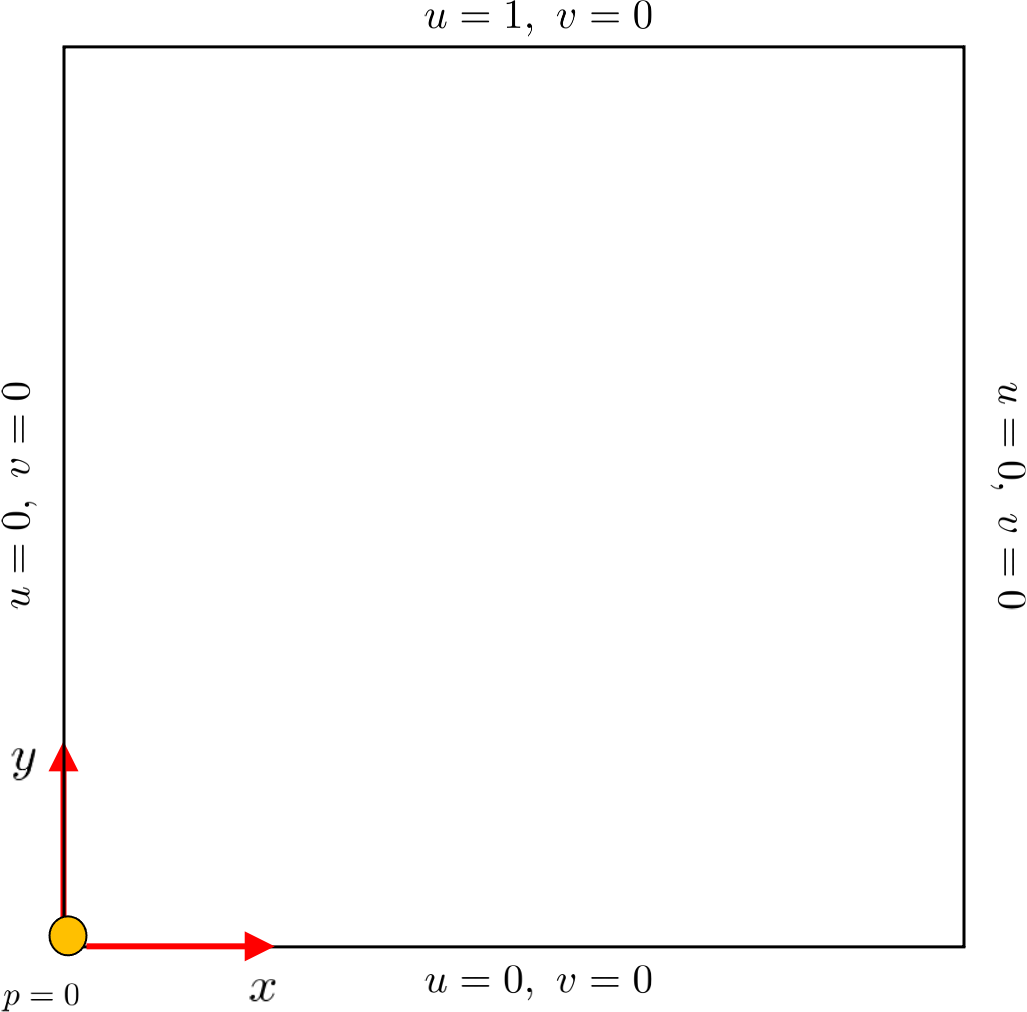
\includegraphics[width=0.5\textwidth]{boundary}	
    \caption{Domain and boundary condition for cavity flow}
    \label{domain}
\end{figure}

Figure \ref{domain} represents the domain with extent  $[0, 1]\otimes[0,1]$ and no-slip boundary conditions are applied at left, bottom and right boundaries.
The top boundary is moving with constant velocity in the positive x direction. The solutions of $\bm{u}=[u,v]$ and $p$ for $Re=100$ is given in Figure 2.
\begin{figure}
	\centering
    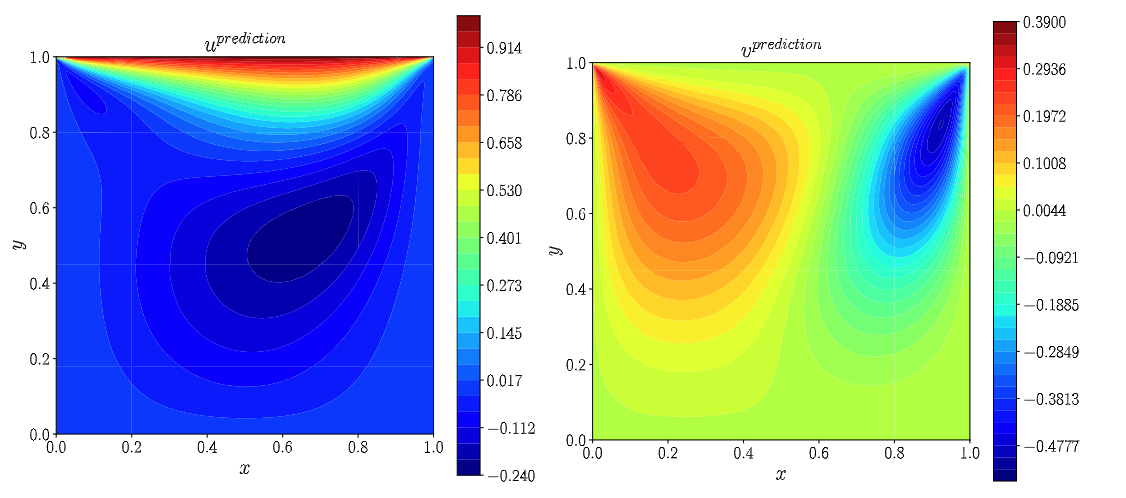
\includegraphics[width=\textwidth]{cflow.png}	
    \caption{$u,v$, and $p$ for a lid driven cavity flow}
    \label{domain}
\end{figure}

\section*{Dataset}
The data for $\bm{u}$ obtained by solving the \autoref{eq1} using spectral element method is provided. The data is provided in ``.mat'' format. The data can be loaded using \textit{scipy} package of python, e.g. \textit{scipy.io.loadmat}.

\textbf{Important:} You may use LLMs for \emph{programming assistance only}. All physical reasoning, mathematical arguments, diagnostics, and interpretation must be your own. Grading emphasizes understanding of incompressibility, boundary layers, and reconstruction limits.

\subsection*{Task 0: Physics audit for cavity flow (required)}
\begin{enumerate}
\item Describe the expected qualitative structure of the $\mathrm{Re}=100$ cavity flow: primary recirculation cell, secondary corner eddies, and shear layer near the moving lid. Indicate which features are driven primarily by boundary conditions vs. nonlinear advection.
\item Explain why pressure is only determined up to an additive constant. Propose a gauge condition you will impose in your PINN implementation and justify it.
\item Write down at least two physically meaningful diagnostics beyond $L^2$ error that you will use in this project (e.g., divergence norm, vorticity extrema, centerline velocity profiles).
\end{enumerate}

\subsection*{Task 1: Forward problem --- solve with PINNs}
\begin{enumerate}
\item Train a PINN to solve the steady cavity problem at $\mathrm{Re}=100$ using only the PDE residuals and boundary conditions.
\item Validate your solution by plotting:
\begin{itemize}
\item $u(x,y)$ and $v(x,y)$ contour plots,
\item vorticity $\omega=\partial_x v-\partial_y u$,
\item centerline profiles $u(x,0.5)$ and $v(0.5,y)$.
\end{itemize}
\item Compare your centerline profiles with those computed from the provided spectral-element dataset. Report relative $L^2$ errors for $u$ and $v$.
\item \textbf{Failure-mode check (core):} Provide one example of a visually plausible PINN solution that is physically wrong (e.g., violates incompressibility locally or smears the lid shear layer). Give a diagnostic that detects it.
\end{enumerate}

\subsection*{Task 2: Reconstruction from sparse interior data}
\begin{enumerate}
\item Randomly sample $N=10,20,30,40$ points inside a fixed interior patch for measurements of $u,v$ and $p$.
\item Reconstruct $u,v,p$ over the entire domain using a PINN with data loss + PDE residual + boundary conditions.
\item Report relative $L^2$ errors for $u$, $v$, and $p$ separately. Also report the divergence norm $\|\nabla\cdot\mathbf{u}\|_{L^2}$.
\item Plot error heatmaps and explain where (spatially) reconstruction fails first as $N$ decreases (e.g., near corners, lid shear layer), and why.
\end{enumerate}

\subsection*{Task 3: Sampling strategy and patch location}
\begin{enumerate}
\item Compare two sampling strategies within the same patch: (i) uniform random sampling and (ii) Latin Hypercube Sampling (LHS).
\item Move the patch to two different locations: (A) near the center recirculation region, (B) near the lid shear layer.
\item For fixed $N$, compare reconstruction quality across these patch locations. Use your diagnostics from Task~0 to explain which region provides more information about the global flow.
\end{enumerate}

\subsection*{Task 4: Noise robustness and regularization}
\begin{enumerate}
\item Add synthetic noise (1\%, 5\%) to the interior measurements and repeat Task~2.
\item Propose and implement one robustness modification (e.g., Huber loss for data, adaptive residual weighting, smoothing/denoising of inputs, or collocation resampling).
\item Quantify how the modification changes reconstruction error and divergence error.
\end{enumerate}

\subsection*{Task 5: Sensitivity to Reynolds number (conceptual)}
\begin{enumerate}
\item Explain how the solution is expected to change qualitatively as $\mathrm{Re}$ increases from 100 to 1000 (e.g., thinner boundary layers, stronger corner eddies).
\item If you had sparse data at an unknown Reynolds number, what would be your strategy to infer $\mathrm{Re}$? State what data (and where) would be most informative.
\end{enumerate}

\section*{Submission requirements}
\begin{itemize}
\item A report (8--10 pages) emphasizing: physics diagnostics, reconstruction limits, sampling/patch effects, and failure modes.
\item Include contour plots, vorticity, centerline profiles, error heatmaps, and divergence diagnostics.
\item Code may be assisted by LLMs; the written analysis must reflect your own understanding.
\end{itemize}

\begin{figure}[!htb]
	\centering
    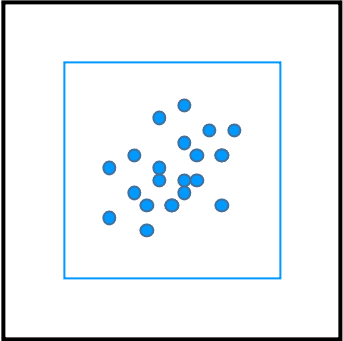
\includegraphics[width=0.35\textwidth]{Patch.png}	
    \caption{An example of patch and sample strategy.}
    \label{domain}
\end{figure}


\subsection*{Programming Options}
You may use \href{https://www.tensorflow.org/}{TensorFlow}, \href{https://pytorch.org/}{PyTorch}, \href{https://deepxde.readthedocs.io/en/latest/}{DeepXDE} or \href{https://developer.nvidia.com/modulus}{Modulus} for completing the tasks.

% \bibliographystyle{abbrv}
% \bibliography{ref}

\end{document}
